\documentclass[12pt]{article}
\usepackage{amsmath}
\usepackage{graphicx,psfrag,epsf}
\usepackage{enumerate}
\usepackage{natbib}
\usepackage{url} 
\usepackage{color, colortbl}

\usepackage{geometry}
\geometry{margin=1in}


\usepackage{amsmath,amsfonts}
\usepackage{mathrsfs,color,nicefrac,multirow,colortbl}

\newcommand{\etal}{\textit{et al.}}
\newcommand{\inc}[2]{ \ifthenelse{\equal{#1}{1}}{\input{./sections/#2}}{ } }
\definecolor{Gray}{gray}{0.9}

\begin{document}


	\begin{center}
		\textbf{Supplemental Figures for \\ ``A Structured Framework for Adaptively Incorporating External\\ 
		         Evidence in Sequentially Monitored Clinical Trials''} \\

		\vspace{1cm}
			Evan Kwiatkowski\textsuperscript{1}, Eugenio Andraca-Carrera\textsuperscript{2}, 
			Mat Soukup\textsuperscript{2}, Matthew A. Psioda\textsuperscript{1}\\

		\vspace{1cm}
			\textsuperscript{1} Department of Biostatistics, University of \\
			North Carolina, McGavran-Greenberg Hall, CB\#7420 \\

		\vspace{1cm}
			\textsuperscript{2}XXXX
	\end{center}

\renewcommand\thefigure{S\arabic{figure}}   


\newpage
\begin{figure}[h]
		\centering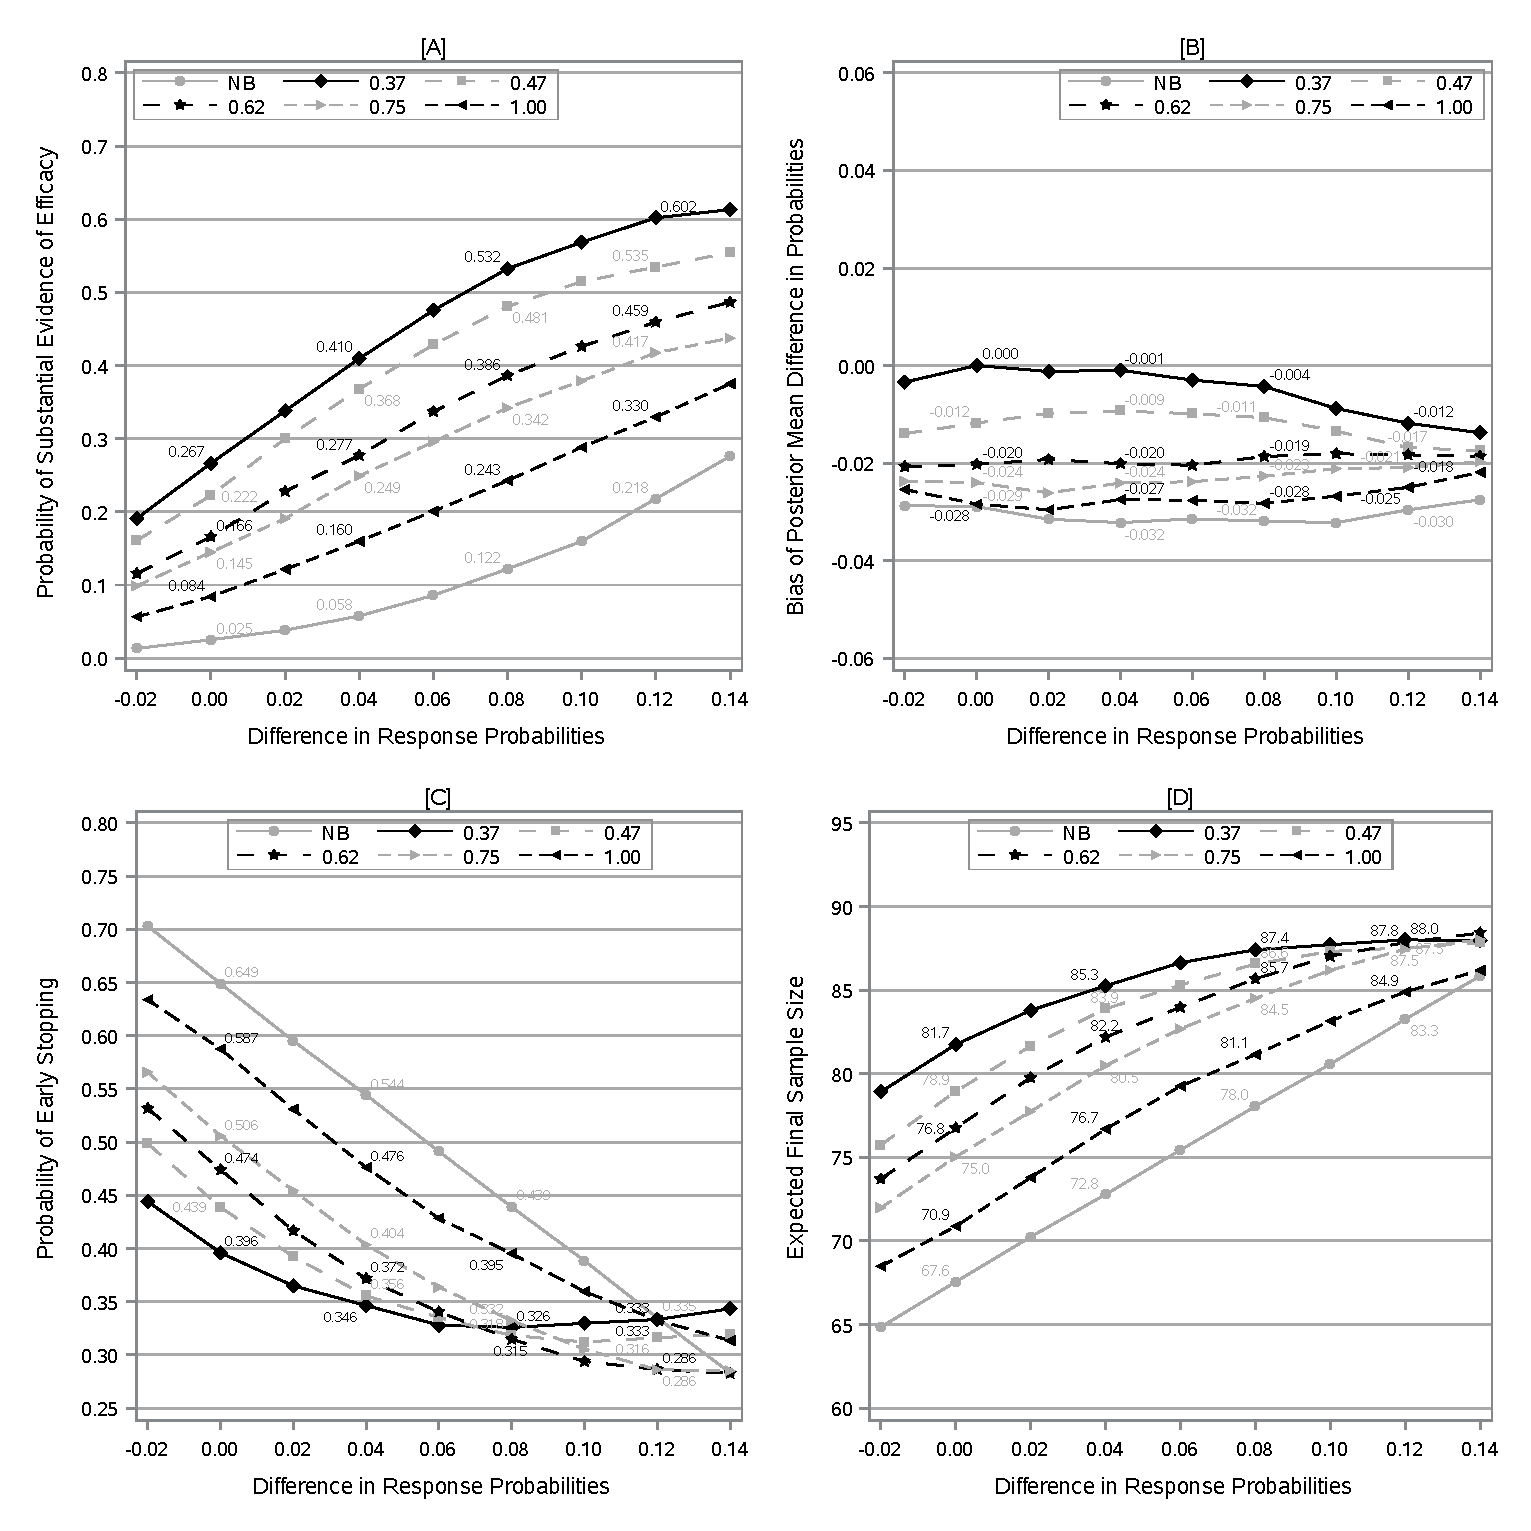
\includegraphics[scale=0.65]{./figures/PLUTO-POWER-2STAGE-FIGC.pdf}  
		\caption{Panel A-D present the probability of obtaining substantial evidence of efficacy,
		         the bias of the posterior mean difference in response probabilities, the probability
						 of early stopping, and the expected sample size, respectively. Selected values
						 are annotated above the scatter plot points. Results based on a control group response
						 probability equal to 0.43.} \label{POWER2}
						
\end{figure}	

\end{document}